\documentclass[crop,tikz]{standalone}
\usepackage{pgfplots}
\usepackage{tikz-3dplot}
\begin{document}

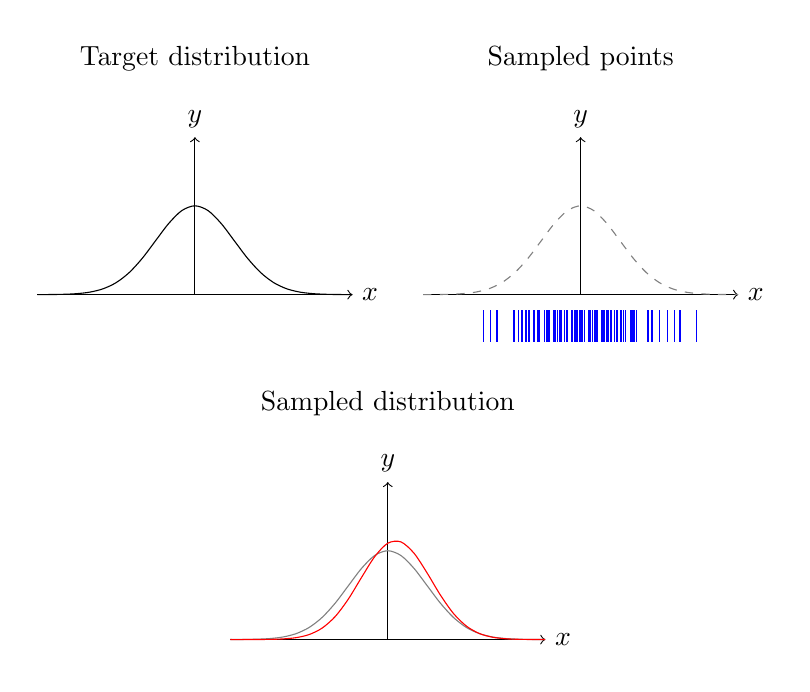
\begin{tikzpicture}[
  declare function={mu1=0;},
  declare function={sigma1=1;},
  declare function={normal(\x,\m,\s)=1/(2*\s*sqrt(pi))*exp(-(\x-\m)^2/(2*\s^2));},
  declare function={invnormal(\x)=0.3*ln(\x/(1-\x));}, % aprox. using logit(x)
  ]
\matrix[column sep=-20mm, row sep=5mm] {
\begin{scope}[yscale=2]
  \draw[->] (-2,0) -- (2,0) node[right] {$x$};
  \draw[->] (0,0) -- (0,1) node[above] {$y$};
  \draw[domain=-2:2,smooth,variable=\x,black] plot (\x,{normal(\x,0,0.5)});
  \node [black] at (0, 1.5) {Target distribution};
\end{scope}
&
&
\begin{scope}[yscale=2]
  \draw[->] (-2,0) -- (2,0) node[right] {$x$};
  \draw[->] (0,0) -- (0,1) node[above] {$y$};
  \foreach \i in {1,2,...,100} {
    \pgfmathsetmacro{\t}{0.5+0.5*rand}
    \draw[blue] ({invnormal(\t)},-0.1) -- ({invnormal(\t)},-0.3);
  }
  \draw[dashed,domain=-2:2,smooth,variable=\x,gray] plot (\x,{normal(\x,0,0.5)});
  \node [black] at (0, 1.5) {Sampled points};
\end{scope}
\\
&
\begin{scope}[yscale=2]
  \draw[->] (-2,0) -- (2,0) node[right] {$x$};
  \draw[->] (0,0) -- (0,1) node[above] {$y$};
  \draw[domain=-2:2,smooth,variable=\x,gray] plot (\x,{normal(\x,0,0.5)});
  \draw[domain=-2:2,smooth,variable=\x,red] plot (\x,{normal(\x,0.1,0.45)});
  \node [black] at (0, 1.5) {Sampled distribution};
\end{scope}
&
\\
};
\end{tikzpicture}

\end{document}